\section{Architecture}
\subsection{Process architecture}
\begin{center}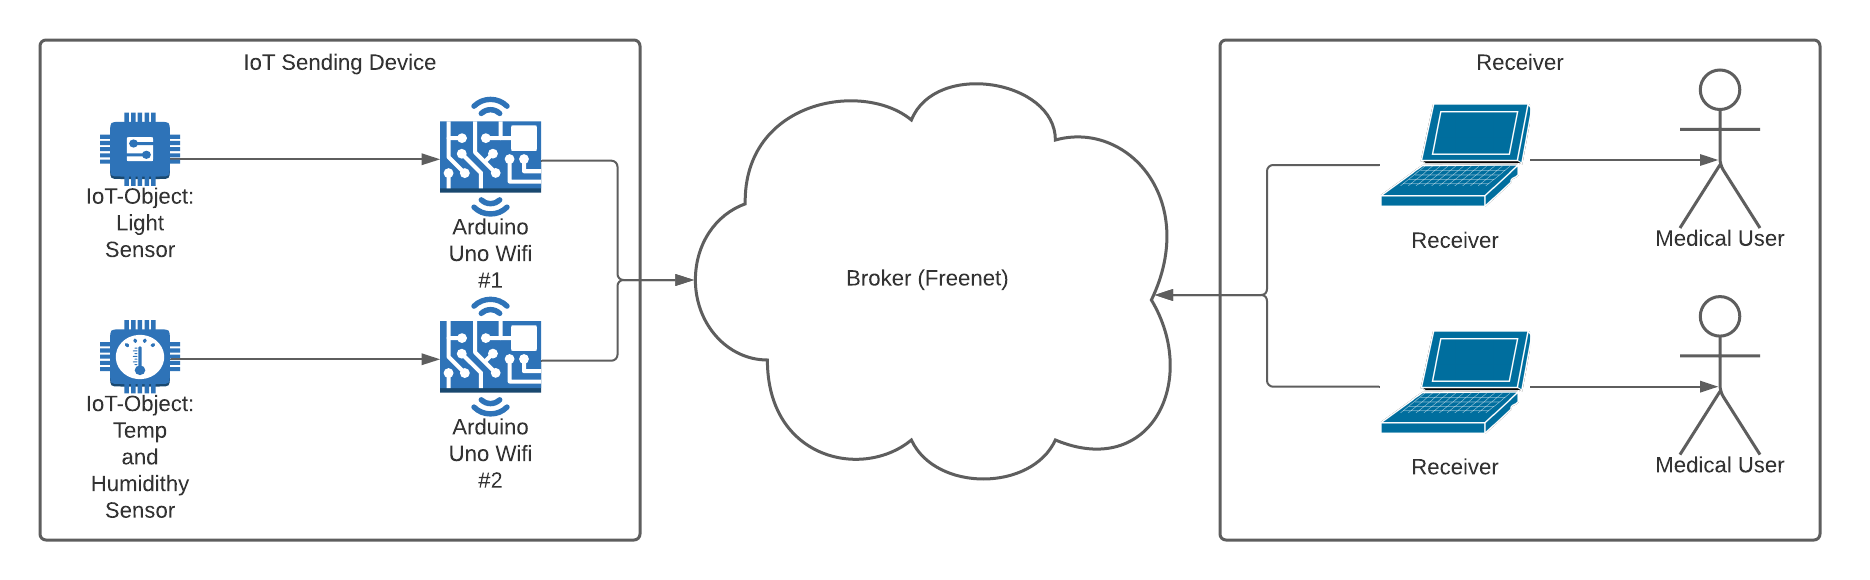
\includegraphics[width=12cm,height=15cm,keepaspectratio]{Architecture}\end{center}

\subsection{Initialization of the communication}
In order for communication to be established between the devices, they must exchange data.
In order to be able to exchange data, each device will come with a scratchable QR Code on it.
This QR Code will contain a key which will be used to send Data to this device on Freenet.
\newline
After the Key is registered at an other device, the two devices need to exchange the connection information.
They start by creating an Key for encryption and decryption of informationen, second they share the specific path's for freenet where data can be send from each device to the other.
\newpage

\begin{landscape}
\subsubsection{Initialization of communication}
\scalebox{0.7}{
\tcbox[top=0pt,left=0pt,right=0pt,bottom=0pt]{
\pseudocodeblock{
 \textbf{IoT sender} \< \< \textbf{Broker} \< \< \textbf{IoT receiver} \\[][\hline]
  \< \< \< \< \text{Register sender Freenet path } \\
  \< \< \< \sendmessageleft{top=Upload receiver Freenet path} \< \\
  \< \< \text{store receiver path} \< \< \\
  \< \sendmessageright{top=Get receiver path} \< \< \< \\
  \< \sendmessageleft{top=return receiver path} \< \< \< \\
  \text{Register receiver Freenet path} \< \< \< \< \\
\text{Gen random ECC key pair}  \< \< \< \< \text{Gen random ECC key pair} \\
 \< \sendmessageright{top=Upload sender pubkey} \< \< \sendmessageleft{top=upload receiver pubkey} \< \\
 \< \< \text{store information} \< \< \\
 \< \sendmessageleft{top=get receiver pubkey} \< \< \sendmessageright{top=get sender pubkey} \< \\
   \text{Calculate shared secret} \< \< \< \< \text{Calculate shared secret} \\
 \text{Gen new SSK Keypair} \< \< \< \< \text{Gen new SSK Keypair} \\
 \text{(Freenet path)} \< \< \< \< \text{(Freenet path)} \\
 \text{Encrypt Freenet path} \< \< \< \< \text{Encrypt Freenet path} \\
 \< \sendmessageright{top=Upload Freenet path} \< \< \sendmessageleft{top=Upload Freenet path} \< \\
 \< \< \text{store information} \< \< \\
 \< \sendmessageleft{top=get Freenet path} \< \< \sendmessageright{top=get Freenet path} \< \\
 \text{store receiver Freenet path} \< \< \< \< \text{store sender Freenet path} \\
}
}
}

\subsubsection{Send and receive data}
\centering
\scalebox{0.7}{
\tcbox[top=0pt,left=0pt,right=0pt,bottom=0pt]{
\pseudocodeblock{
 \textbf{IoT sender} \< \< \textbf{Broker} \< \< \textbf{IoT receiver} \\[][\hline]
 \text{Get stored Freenet path} \< \< \< \< \\
 \text{Get shared secret} \< \< \< \< \\
 \text{Encrypt information} \< \< \< \< \\
 \< \sendmessageright{top=Upload info} \< \< \< \\
 \< \<  \text{store info} \< \< \\
 \< \sendmessageleft{top=Upload result} \< \< \< \\
 \< \< \< \sendmessageright{top=Get info} \< \\ 
 \< \< \< \< \text{Get shared secret} \\
 \< \< \< \< \text{Decrypt information} \\
  \< \< \< \< \text{Get stored Freenet path} \\
 \< \< \< \< \text{Encrypt receive confirmation} \\
 \< \< \< \sendmessageleft{top=Send receive confirmation} \< \\
 \< \<  \text{store receive confirmation} \< \< \\
 \< \sendmessageleft{top=get receive confirmation} \< \< \< \\
 \text{Get shared secret} \< \< \< \< \\
 \text{start over} \< \< \< \< \\
}
}
}
\end{landscape}